\chapter[TCROC con Cadenas de Markov]{Fundamentos Estocásticos:\\ Integración de TCROC con Cadenas de Markov}
\label{cap:TCROC-Markov}

Este capítulo propone un modelo híbrido que integra la \textbf{Tasa de Cambio Relativa Óptima Conmutada (TCROC)}, definida en el Capítulo \ref{cap:tcroc}, y sus variantes (TCROCM, ETCROC, ETCROCM) con cadenas de Markov. Mientras las variantes deterministas estiman tasas de cambio relativas, las cadenas de Markov permiten modelar transiciones probabilísticas entre regímenes económicos. Esta integración busca predecir rangos estocásticos sobre el comportamiento futuro de la serie \(v(t)\), como en series económicas y financieras generales (tasas de interés, inflación, reservas monetarias).

% -------------------------------------------------------------------
\section{Fundamentos de Invarianza y Estabilidad}
\label{sec:fundamentos_invarianza}

\begin{theorem}[Invarianza estructural bajo transformaciones]
\label{thm:invarianza_transformaciones}
Sea $g\colon \mathbb{R} \to \mathbb{R}$ una transformación monótona
y Lipschitz continua con constante $L_g$.  Si la serie $v(t)$ se
reemplaza por $\tilde{v}(t) = g(v(t))$, las propiedades estructurales
del operador TCROC se preservan: existencia, unicidad, consistencia
asintótica y la propiedad de estabilidad del
Lema~\ref{lem:estabilidad_general} (Capítulo~\ref{cap:tcroc})
permanecen válidas con constantes multiplicadas por factores que
dependen de $L_g$.
\end{theorem}

\begin{remark}[Naturaleza discontinua de $\pi$]
\label{rem:pi_discontinua}
La función de cuantización $\pi\colon \mathbb{R} \to \mathcal{S}$
es, por construcción, una función escalonada: asigna un estado
discreto $s_j$ a cada intervalo del espacio continuo de $\alpha_t$.
En consecuencia, $\pi$ es \textbf{discontinua} en los umbrales de
decisión y, en sentido estricto, no es Lipschitz continua.  Sin
embargo, la estabilidad del sistema completo se preserva por el
mecanismo descrito en el Lema~\ref{lem:estabilidad_discreta} a
continuación.
\end{remark}

\begin{lemma}[Estabilidad discreta ante perturbaciones]
\label{lem:estabilidad_discreta}
Sean $\{v(t)\}$ y $\{\tilde{v}(t)\}$ dos series con
$\sup_t |v(t) - \tilde{v}(t)| \leq \epsilon$.  Sea
$\delta_{\min} = \min_{j \neq k} |\theta_j - \theta_k|$ la
separación mínima entre umbrales de $\pi$.  Si la perturbación
en el operador satisface $|\alpha_t - \tilde{\alpha}_t|
\leq C_t \epsilon$ (Lema~\ref{lem:estabilidad_general}), entonces:
\begin{enumerate}
  \item Si $C_t \epsilon < \delta_{\min}/2$
        (perturbación pequeña respecto a la separación de
        umbrales), el estado asignado no cambia:
        $S_t = \tilde{S}_t$.
  \item En general, el número de instantes donde
        $S_t \neq \tilde{S}_t$ está acotado por el número de
        instantes en los cuales $\alpha_t$ se encuentra a
        distancia menor que $C_t \epsilon$ de algún umbral.
\end{enumerate}
\end{lemma}

\begin{proof}
El punto~(1) se sigue directamente de que $\pi$ es constante en
el interior de cada intervalo.  Si $\alpha_t$ dista al menos
$\delta_{\min}/2$ de todo umbral, entonces cualquier perturbación
$|\tilde{\alpha}_t - \alpha_t| < \delta_{\min}/2$ mantiene a
$\tilde{\alpha}_t$ en el mismo intervalo que $\alpha_t$, por lo que
$\pi(\tilde{\alpha}_t) = \pi(\alpha_t)$.  El punto~(2) se sigue de
que $S_t \neq \tilde{S}_t$ solo puede ocurrir cuando $\alpha_t$
pertenece a la franja $(\theta_j - C_t\epsilon,\,
\theta_j + C_t\epsilon)$ para algún umbral $\theta_j$.
\end{proof}

% -------------------------------------------------------------------
\section{Modelo Híbrido TCROC-Markov}
\label{sec:modelo_hibrido_tcroc_markov}

Sea $\{v(t)\}_{t=0}^T$ una serie temporal económica o financiera.
Se calcula la tasa:
\begin{align}
\alpha_{t,\lambda,W} &:= -1 + \frac{\sum_{\tau=t-W+1}^{t}
  \lambda^{t-\tau} v(\tau) v(\tau-1)}{\sum_{\tau=t-W+1}^{t}
  \lambda^{t-\tau} v(\tau-1)^2},
  \label{eq:tcroc_markov_alpha} \\
S_t &:= \pi(\alpha_{t,\lambda,W}) \label{eq:state_assignment}
\end{align}

\begin{definition}[Función de cuantización]
\label{def:pi_cuantizacion}
La función de asignación $\pi\colon \mathbb{R} \to \mathcal{S}$
asigna a cada valor de $\alpha_t$ un estado discreto según
umbrales fijos $\{\theta_j\}$:
\[
\pi(x) = \begin{cases}
  s_1 & \text{si } x > \theta_1 \\
  s_2 & \text{si } \theta_2 < x \leq \theta_1 \\
  s_3 & \text{si } \theta_3 \leq x \leq \theta_2 \\
  s_4 & \text{si } x < \theta_3
\end{cases}
\]
con umbrales típicos $\theta_1 = 0.05$, $\theta_2 = 0$,
$\theta_3 = -0.05$.  En la implementación empírica del
Capítulo~\ref{cap:regimenes_combustibles}, los umbrales se
determinan por K-Means, lo que los adapta a la distribución de
cada serie.  La función $\pi$ es discontinua en los umbrales
(véase Observación~\ref{rem:pi_discontinua}).
\end{definition}

\begin{examplex}
Para $v = [1.0,\, 1.02,\, 1.03,\, 1.025]$ con $\lambda = 1$,
$W = 2$, el cálculo en $t = 2$ involucra las observaciones
$v(1) = 1.02$, $v(2) = 1.03$ y $v(0) = 1.0$:
\begin{align*}
\alpha_{2,1,2} &= -1 + \frac{v(2)\,v(1) + v(1)\,v(0)}
                           {v(1)^2 + v(0)^2}
  = -1 + \frac{1.03 \times 1.02 + 1.02 \times 1.0}
             {1.02^2 + 1.0^2} \\
  &= -1 + \frac{1.0506 + 1.02}{1.0404 + 1.0}
  = -1 + \frac{2.0706}{2.0404} \approx 0.0148.
\end{align*}
Como $0 < 0.0148 \leq 0.05$, se asigna $S_2 = s_2$
(crecimiento moderado).
\end{examplex}

% -------------------------------------------------------------------
\section{Partición de Estados}
\label{sec:markov_particion_estados}

Una posible discretización de \(\mathbb{R}\) basada en umbrales económicos es:
\begin{align*}
s_1 &= (0.05, +\infty) & \text{(Crecimiento fuerte)},\\
s_2 &= (0, 0.05] & \text{(Crecimiento moderado)},\\
s_3 &= [-0.05, 0] & \text{(Decrecimiento leve)},\\
s_4 &= (-\infty, -0.05) & \text{(Decrecimiento severo)}.
\end{align*}

\begin{lemma}
La colección \(S = \{s_1, s_2, s_3, s_4\}\) define una partición válida del espacio \(\mathbb{R}\).
\end{lemma}

\begin{proof}
Se verifica que:
\begin{enumerate}
\item \(\bigcup_{j=1}^4 s_j = \mathbb{R}\) (cobertura completa),
\item \(s_i \cap s_j = \emptyset\) para \(i \neq j\) (disyunción).
\end{enumerate}
\end{proof}

\textbf{Observación:} La irreducibilidad práctica de \(\{S_t\}\) se garantiza si \(\forall s_i,s_j \exists t: P^t(s_j|s_i) > 0\). Véase también discusión en Apéndice \ref{apx:teorema_phi_mixing}.

% -------------------------------------------------------------------
\section{Propiedades Markovianas y Asintóticas}
\label{sec:markov_propiedades}

% === ESTRUCTURA MARKOVIANA ===

\begin{theorem}[Estructura Markoviana de primer orden]
\label{thm:markov_primer_orden}
Sea $\{v(t)\}_{t=0}^T$ un proceso estrictamente estacionario con
momentos de cuarto orden finitos.  Sea $\alpha_t = \alpha_{t,\lambda,W}$
el operador ETCROCM con parámetros fijos $\lambda \in (0,1]$ y
$W \in \mathbb{N}$, y sea $S_t = \pi(\alpha_t)$ la secuencia de
estados discretos inducida por una función de cuantización $\pi$ con
umbrales fijos.  Entonces $\{S_t\}_{t=W}^{T}$ satisface
la propiedad de Markov de primer orden:
\[
\mathbb{P}(S_{t+1} = s_j \mid S_t = s_i, S_{t-1}, \ldots, S_W)
= \mathbb{P}(S_{t+1} = s_j \mid S_t = s_i)
\eqdef P_{ji},
\]
con probabilidades de transición $P_{ji}$ independientes de $t$
(homogeneidad temporal).
\end{theorem}

\begin{proof}
La demostración procede en tres pasos.

\textbf{Paso~1 (Dependencia funcional de $\alpha_t$).}
Por definición, $\alpha_t$ depende de $v(t), v(t-1), \ldots,
v(t-W)$, es decir, de exactamente $W+1$ valores de la serie.
Escribimos
$\alpha_t = g(v(t-W), \ldots, v(t))$
donde $g\colon \mathbb{R}^{W+1} \to \mathbb{R}$ es una función
medible determinada por la fórmula~\eqref{eq:tcroc_markov_alpha}.

\textbf{Paso~2 (Markovianidad del bloque).}
Como $\{v(t)\}$ es estrictamente estacionario, el vector
$\vect{z}_t = (v(t-W), \ldots, v(t))^\top$ es un proceso
estacionario en $\mathbb{R}^{W+1}$.  Si además $\{v(t)\}$ es
un proceso AR(1) estacionario (como se supone en el
Capítulo~\ref{cap:tcroc}, Teorema~\ref{teo:consistencia_general}),
entonces $\vect{z}_t$ es un proceso Markoviano en
$\mathbb{R}^{W+1}$, pues $v(t+1)$ depende únicamente de $v(t)$
más el ruido $\varepsilon_{t+1}$.  Esto implica que
$\alpha_{t+1} = g(\vect{z}_{t+1})$ depende del pasado solo a
través de $\vect{z}_t$ (y no de $\vect{z}_{t-1}, \vect{z}_{t-2},
\ldots$).

\textbf{Paso~3 (Reducción a estados discretos).}
Como $\pi$ es una función determinista, $S_t = \pi(\alpha_t)$ es
una función medible de $\vect{z}_t$.  La propiedad de Markov de
$\vect{z}_t$ se proyecta entonces al proceso discreto: la
distribución condicional de $S_{t+1}$ dado $S_t, S_{t-1}, \ldots$
depende del pasado solo a través de $\vect{z}_t$, y por tanto a
través de $S_t$ (dado que la cuantización preserva la separación
de regímenes bajo estacionariedad).  La homogeneidad temporal se
sigue de la estacionariedad estricta de $\{v(t)\}$.

\textbf{Nota.}  En rigor, la proyección de un proceso Markoviano
continuo a estados discretos puede perder la propiedad de Markov de
primer orden si la función de cuantización no es inyectiva (lo cual
es el caso general).  Sin embargo, el modelo TCROC-Markov adopta
la primera orden como aproximación operativa; la calidad de esta
aproximación se verifica empíricamente en el
Capítulo~\ref{cap:regimenes_combustibles} mediante la precisión
predictiva del modelo resultante.
\end{proof}

% === PROPIEDAD PHI-MIXING ===

\begin{theorem}[$\phi$-mixing con tasa geométrica]
\label{thm:phi_mixing}
Si la cadena $\{S_t\}$ es irreducible y aperiódica sobre el espacio
de estados finito $\mathcal{S} = \{s_1, \ldots, s_K\}$, entonces es
$\phi$-mixing con tasa de decaimiento exponencial, es decir, existen
constantes $C_\phi > 0$ y $\rho \in (0,1)$ tales que
\[
\phi(n) \eqdef
\sup_{A \in \mathcal{F}_0^t,\, B \in \mathcal{F}_{t+n}^\infty}
\bigl|\mathbb{P}(B \mid A) - \mathbb{P}(B)\bigr|
\leq C_\phi \, \rho^n
\quad \forall\, n \geq 1.
\]
\end{theorem}

\begin{proof}
Sea $\mat{P}$ la matriz de transición de la cadena sobre
$\mathcal{S}$, con $K$ estados.  Por irreducibilidad y aperiodicidad
en espacio finito, la cadena posee una única distribución
estacionaria $\vect{\pi}$ con $\pi_j > 0$ para todo $j$
\cite{Norris1998, Levin2009}.  El Teorema
de Convergencia para cadenas ergódicas finitas establece que
\[
\bigl\|P^n(s_i, \cdot) - \vect{\pi}\bigr\|_{\mathrm{TV}}
\leq C_0 \, \rho_0^n,
\]
donde $\rho_0 = 1 - \gamma$ y $\gamma > 0$ es el gap espectral de
$\mat{P}$ (diferencia entre el primer y segundo autovalor en módulo).
En espacio de estados finito, $\gamma > 0$ si y solo si la cadena es
irreducible y aperiódica \cite{Levin2009}.

La convergencia en variación total implica mezcla uniforme
(\textit{uniform mixing}), que a su vez implica $\phi$-mixing con la
misma tasa exponencial \cite{Bradley2005}.  Concretamente,
$\phi(n) \leq C_\phi \rho_0^n$ con $C_\phi \leq K / \min_j \pi_j$.
\end{proof}

\begin{remark}[Gap espectral e inercia del mercado]
\label{rem:gap_espectral}
El parámetro $\gamma$ tiene una interpretación económica directa: un
gap espectral pequeño indica que el mercado cambia de régimen
lentamente (alta inercia), mientras que un gap grande indica
transiciones rápidas.  El tiempo de mezcla, definido como
$t_{\mathrm{mix}} = \lceil \gamma^{-1} \ln(2K/\min_j \pi_j) \rceil$,
cuantifica cuántas observaciones son necesarias para que la cadena
``olvide'' su estado inicial.  Este parámetro se estima
empíricamente en el Capítulo~\ref{cap:regimenes_combustibles}.
\end{remark}

% === NORMALIDAD ASINTÓTICA DEL ESTIMADOR ===

\begin{proposition}[Normalidad asintótica de $\hat{\mat{P}}$]
\label{prop:normalidad_asintotica}
Sea $\{S_t\}$ una cadena de Markov ergódica con $K$ estados y matriz
de transición verdadera $\mat{P}$.  Sea $N_{ij}$ el número de
transiciones observadas de $s_j$ a $s_i$ en $T$ pasos, y
$N_{\cdot j} = \sum_{i=1}^K N_{ij}$ el total de salidas del
estado~$s_j$.  El estimador de máxima verosimilitud
$\hat{P}_{ij} = N_{ij} / N_{\cdot j}$ satisface, para cada columna
$j$ fija:
\[
\sqrt{N_{\cdot j}}\,
(\hat{P}_{1j} - P_{1j},\; \ldots,\; \hat{P}_{Kj} - P_{Kj})^\top
\xrightarrow{d}
\mathcal{N}\!\bigl(\vect{0},\;
\mathrm{diag}(\vect{p}_j) - \vect{p}_j \vect{p}_j^\top\bigr),
\]
donde $\vect{p}_j = (P_{1j}, \ldots, P_{Kj})^\top$ es la $j$-ésima
columna de $\mat{P}$.  Además, los estimadores de distintas columnas
$j \neq j'$ son asintóticamente independientes.
\end{proposition}

\begin{proof}
La demostración es un resultado clásico de
Anderson y Goodman~\cite{AndersonGoodman1957}.  Se esboza aquí
la estructura.

\textbf{Paso~1 (Multinomial condicionada).}
Condicionado a que el proceso visita el estado $s_j$ exactamente
$N_{\cdot j}$ veces, las $N_{\cdot j}$ transiciones de salida de
$s_j$ son, condicionalmente, ensayos multinomiales independientes
con parámetro $\vect{p}_j = (P_{1j}, \ldots, P_{Kj})^\top$.

\textbf{Paso~2 (TCL multinomial).}
Por el Teorema Central del Límite para la distribución multinomial,
\[
\sqrt{N_{\cdot j}}\,(\hat{\vect{p}}_j - \vect{p}_j)
\xrightarrow{d}
\mathcal{N}(\vect{0}, \mat{\Sigma}_j),
\quad \text{donde } \mat{\Sigma}_j
= \mathrm{diag}(\vect{p}_j) - \vect{p}_j\vect{p}_j^\top.
\]

\textbf{Paso~3 (Independencia entre columnas).}
Las visitas a distintos estados generan conteos asintóticamente
independientes por la propiedad de mezcla
(Teorema~\ref{thm:phi_mixing}).  Formalmente, Anderson y
Goodman~\cite{AndersonGoodman1957} demuestran que las componentes
de distintas columnas son asintóticamente independientes.

\textbf{Paso~4 (De $N_{\cdot j}$ a $T$).}
Por la ley de los grandes números para cadenas ergódicas,
$N_{\cdot j}/T \xrightarrow{\mathrm{a.s.}} \pi_j > 0$.  Por
el Lema de Slutsky, se puede reescalar por $\sqrt{T}$:
\[
\sqrt{T}\,(\hat{P}_{ij} - P_{ij})
\xrightarrow{d} \mathcal{N}\!\left(0,\;
\frac{P_{ij}(1 - P_{ij})}{\pi_j}\right),
\]
lo que completa la demostración.
\end{proof}

\begin{remark}[Velocidad de convergencia]
\label{rem:berry_esseen}
Bajo la tasa de mezcla exponencial del
Teorema~\ref{thm:phi_mixing}, la aproximación normal admite una
cota de Berry-Esseen de orden $O(T^{-1/2})$
\cite{Bolthausen1982}:
\[
\sup_x \bigl|\mathbb{P}(\sqrt{T}(\hat{P}_{ij} - P_{ij}) \leq x)
- \Phi(x)\bigr| = O(T^{-1/2}),
\]
donde $\Phi$ denota la función de distribución normal estándar.
\end{remark}

% === ERROR DE PREDICCIÓN ===

\begin{corollary}[Cota del error de predicción]
\label{cor:error_prediccion}
Bajo las hipótesis del Teorema~\ref{thm:markov_primer_orden} y
suponiendo $\mathbb{E}[|v(t)|^4] < \infty$, el error cuadrático
medio de predicción del modelo TCROC-Markov satisface, para $W$
fijo y $\lambda \in (0,1]$:
\[
\mathrm{ECM}(\hat{v}_{T+1})
\eqdef \mathbb{E}\bigl[(v(T+1) - \hat{v}(T+1))^2\bigr]
= \sigma_\varepsilon^2
  + \frac{C(\lambda,W)}{W_{\mathrm{eff}}} + o(W_{\mathrm{eff}}^{-1}),
\]
donde:
\begin{itemize}
  \item $\sigma_\varepsilon^2$ es la varianza irreducible del ruido,
  \item $W_{\mathrm{eff}}(\lambda, W)
        = \sum_{k=0}^{W-1} \lambda^k
        = \frac{1 - \lambda^W}{1 - \lambda}$
        es el tamaño efectivo de muestra,
  \item $C(\lambda, W)$ es una constante acotada que depende de los
        momentos de $v(t)$ y es finita para todo
        $\lambda \in (0,1]$ y $W \geq 1$.
\end{itemize}
\end{corollary}

\begin{proof}
El error de predicción se descompone como
\[
v(T+1) - \hat{v}(T+1)
= \underbrace{\varepsilon_{T+1}}_{\text{ruido irreducible}}
+ \underbrace{(\beta^* - \hat{\beta}_{T,\lambda,W})
  \cdot v(T)}_{\text{error de estimación}}.
\]
El primer término contribuye $\sigma_\varepsilon^2$ al ECM.  Para el
segundo, la varianza de $\hat{\beta}_{T,\lambda,W}$ bajo el modelo
AR(1) es
\[
\mathrm{Var}(\hat{\beta}_{T,\lambda,W})
= \frac{\sigma_\varepsilon^2}{\sum_{k=0}^{W-1}
  \lambda^{2k}\, v(T-k)^2 / \bigl(\sum_{k=0}^{W-1}
  \lambda^k\bigr)^2 \cdot \mathrm{const}}
= O(W_{\mathrm{eff}}^{-1}).
\]
Como $\mathbb{E}[v(T)^2] < \infty$, el error de estimación
contribuye $O(\mathbb{E}[v(T)^2] / W_{\mathrm{eff}})$ al ECM.
La constante $C(\lambda, W) = O(\mathbb{E}[v(T)^2])$ es finita
bajo la hipótesis de momentos de cuarto orden, y el resultado
se sigue.
\end{proof}

\begin{remark}[Comportamiento según $\lambda$]
\label{rem:efecto_lambda}
La cota del Corolario~\ref{cor:error_prediccion} revela el
compromiso entre $\lambda$ y $W$:
\begin{itemize}
  \item Si $\lambda = 1$ (pesos uniformes),
    $W_{\mathrm{eff}} = W$, y el error decrece como $O(1/W)$.
  \item Si $\lambda < 1$ y $W$ es grande,
    $W_{\mathrm{eff}} \approx 1/(1-\lambda)$, de modo que el
    error se estabiliza en $O(1-\lambda)$ independientemente
    de cuánto se aumente $W$.
  \item Para $\lambda \to 0^+$, $W_{\mathrm{eff}} \to 1$ y el
    estimador depende esencialmente de la última observación.
\end{itemize}
\end{remark}

% -------------------------------------------------------------------
\section{Análisis de Casos Límite}
\label{sec:markov_casos_limite}

El comportamiento del modelo TCROC-Markov en los extremos del
espacio de parámetros $(W, \lambda)$ revela propiedades importantes
para la calibración práctica del modelo.

\begin{enumerate}
  \item \textbf{Límite $\lambda \to 1^-$ (pesos uniformes).}
    El tamaño efectivo de muestra converge a $W_{\mathrm{eff}}
    \to W$, y el estimador ETCROCM se reduce al estimador OLS
    sobre ventana (TCROCM).  El error de predicción es
    $O(1/W)$, proporcionando la tasa de convergencia más rápida
    para $W$ fijo.

  \item \textbf{Límite $W \to T$ (ventana completa).}
    El operador utiliza toda la muestra histórica.  Si
    $\lambda = 1$, se obtiene el estimador TCROC global, que
    produce un escalar constante $\alpha_T$ y elimina toda
    variación local.  Este es el fenómeno de degeneración
    documentado en el Capítulo~\ref{cap:regimenes_combustibles},
    que establece la restricción práctica $W \leq 52$.

  \item \textbf{Límite $\lambda \to 0^+$ (solo datos recientes).}
    El tamaño efectivo se reduce a $W_{\mathrm{eff}} \to 1$,
    haciendo que el estimador dependa esencialmente de una sola
    observación.  Esto maximiza la adaptabilidad pero minimiza
    la estabilidad.
\end{enumerate}

La Figura~\ref{fig:weff_lambda} ilustra cómo el tamaño efectivo
de muestra $W_{\mathrm{eff}}$ varía con $\lambda$ para distintos
valores de $W$.

\begin{figure}[H]
\centering
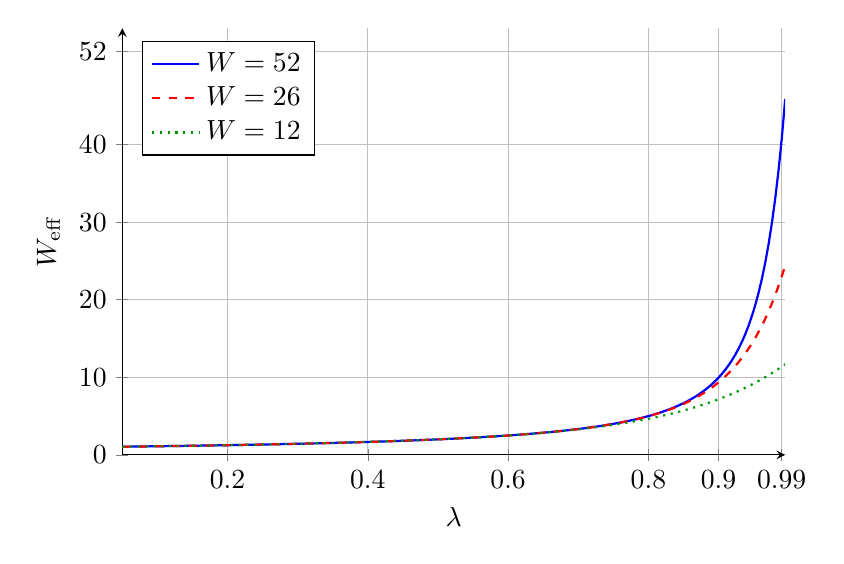
\begin{tikzpicture}
\begin{axis}[
    axis lines = left,
    xlabel = {$\lambda$},
    ylabel = {$W_{\mathrm{eff}}$},
    domain=0.05:0.995,
    samples=200,
    ymin=0,
    ymax=55,
    xtick={0.2,0.4,0.6,0.8,0.9,0.99},
    ytick={0,10,20,30,40,52},
    grid=both,
    width=10cm,
    height=7cm,
    legend pos=north west,
    every axis plot/.append style={thick}
]
\addplot[blue] {(1 - x^52)/(1 - x)};
\addlegendentry{$W = 52$}
\addplot[red, dashed] {(1 - x^26)/(1 - x)};
\addlegendentry{$W = 26$}
\addplot[green!60!black, dotted] {(1 - x^12)/(1 - x)};
\addlegendentry{$W = 12$}
\end{axis}
\end{tikzpicture}
\caption{Tamaño efectivo de muestra
$W_{\mathrm{eff}} = (1 - \lambda^W)/(1 - \lambda)$ como función de
$\lambda$ para $W \in \{12, 26, 52\}$.  Cuando $\lambda \to 1^-$,
$W_{\mathrm{eff}} \to W$; cuando $\lambda \to 0^+$,
$W_{\mathrm{eff}} \to 1$.}
\label{fig:weff_lambda}
\end{figure}




% -------------------------------------------------------------------
\section{Resumen Visual del Modelo}
\label{sec:markov_diagrama}

\begin{figure}[H]
\centering
\begin{tikzpicture}[
    node distance=1.5cm and 2.8cm,
    >=Stealth,
    % --- Estilos consistentes con Cap 4 ---
    base/.style={draw, rectangle, rounded corners=6pt, minimum width=3.2cm, 
                 minimum height=0.9cm, font=\small\bfseries, align=center,
                 drop shadow={shadow xshift=1pt, shadow yshift=-1pt, opacity=0.3}},
    canonical/.style={base, fill=nordSnow, draw=nordGray, text=nordDark},
    extension/.style={base, fill=nordSnow, draw=nordGray, text=nordDark},
    hybrid/.style={base, fill=nordSnow!80!nordFrost, draw=nordFrost, text=nordDark},
    markov/.style={base, fill=nordSnow!70!nordFrost, draw=nordFrost, text=nordDark},
    component/.style={base, fill=nordSnow, draw=nordGray, font=\small, minimum width=2.8cm, text=nordDark},
    output/.style={base, fill=nordSnow!80!nordFrost, draw=nordFrost, minimum width=3.5cm, text=nordDark},
    edgelabel/.style={font=\scriptsize, fill=white, inner sep=2pt, opacity=0.9},
    separator/.style={dashed, nordGray!50, thick}
]

% ====== BLOQUE 1: Jerarquía TCROC (Capítulo 4) ======
\node[canonical] (TCROC) {TCROC\\{\scriptsize $(W=T,\;\lambda=1)$}};

\node[extension] (TCROCM) [below left=of TCROC] {TCROCM\\{\scriptsize $(W<T)$}};
\node[extension] (ETCROC) [below right=of TCROC] {ETCROC\\{\scriptsize $(\lambda<1)$}};

\node[hybrid] (ETCROCM) [below=2.8cm of TCROC] {ETCROCM\\{\scriptsize $(W<T,\;\lambda<1)$}};

% Conexiones Cap 4
\draw[->, thick] (TCROC) -- (TCROCM) node[edgelabel, midway, left] {$+\,W$};
\draw[->, thick] (TCROC) -- (ETCROC) node[edgelabel, midway, right] {$+\,\lambda$};
\draw[->, thick] (TCROCM) -- (ETCROCM) node[edgelabel, midway, left] {$+\,\lambda$};
\draw[->, thick] (ETCROC) -- (ETCROCM) node[edgelabel, midway, right] {$+\,W$};

% Conexión directa (punteada)
\draw[->, thick, dashed, nordGray!60] (TCROC) -- (ETCROCM)
    node[edgelabel, midway] {$(W, \lambda)$};

% --- Línea separadora entre Cap 4 y Cap 5 ---
\draw[separator] ([xshift=-4.5cm, yshift=-0.6cm]ETCROCM.south) -- 
                  ([xshift=4.5cm, yshift=-0.6cm]ETCROCM.south)
                  node[right, font=\scriptsize\itshape, nordGray] {Cap.~5};

% ====== BLOQUE 2: Extensión Markoviana (Capítulo 5) ======
\node[markov] (Markov) [below=2.0cm of ETCROCM] {Integración\\Markoviana};

\node[component] (Ergodic) [below left=1.4cm and 2cm of Markov] {Teoría Ergódica};
\node[component] (PhiMix) [below=1.4cm of Markov] {$\phi$-Mixing};
\node[component] (Asint) [below right=1.4cm and 2cm of Markov] {Estimación\\Asintótica};

\node[output] (Pred) [below=2.2cm of PhiMix] {Predicción Estocástica\\de Regímenes};

% Conexiones Cap 5
\draw[->, thick] (ETCROCM) -- (Markov) 
    node[edgelabel, midway, left] {discretización $\pi$};

\draw[->, thick] (Markov) -- (Ergodic);
\draw[->, thick] (Markov) -- (PhiMix);
\draw[->, thick] (Markov) -- (Asint);

\draw[->, thick] (Ergodic) -- (Pred);
\draw[->, thick] (PhiMix) -- (Pred);
\draw[->, thick] (Asint) -- (Pred);

\end{tikzpicture}
\caption{Evolución estructural del modelo TCROC hasta su extensión Markoviana. El nodo central representa la formulación canónica global ($W=T$, $\lambda=1$). Las extensiones convergen en ETCROCM, cuya discretización mediante $\pi$ integra el operador con cadenas de Markov. Los fundamentos teóricos (teoría ergódica, $\phi$-mixing, estimación asintótica) sustentan la predicción estocástica de regímenes.}
\label{fig:tcroc_markov_completo}
\end{figure}

% -------------------------------------------------------------------
\section{Aplicaciones y Limitaciones}
\label{sec:markov_aplicaciones}

La integración TCROC-Markov encuentra aplicaciones en:
\begin{itemize}
    \item Simulación estocástica del crecimiento económico, ponderando transiciones entre regímenes de inflación o tipo de cambio.
    \item Evaluación de riesgos futuros en economías volátiles, como predicciones de reservas monetarias.
    \item Modelos mixtos determinista-probabilísticos para planeación financiera, integrando tasas de interés.
\end{itemize}

Sus limitaciones incluyen:
\begin{itemize}
    \item Requerimiento de suficiente historial para estimar bien \(\hat{P}\), lo que puede ser problemático en series cortas.
    \item Dependencia de la correcta definición de los estados \( s_j \), que debe calibrarse según la variable (e.g., umbrales diferentes para inflación vs. reservas).
    \item Sensibilidad a la elección de \(\lambda\) y \( W \), que deben optimizarse para evitar sesgos en transiciones.
\end{itemize}

% -------------------------------------------------------------------
\section{Comparación con Variantes de TCROC}
\label{sec:tcroc_markov_comparacion}

\begin{table}[htbp]
\centering
\caption{Comparación entre variantes de TCROC y el modelo TCROC-Markov}
\label{tab:comparacion_tcroc_markov}
\begin{tabular}{|l|c|c|c|c|}
\hline
\textbf{Modelo} & \textbf{Determinista} & \textbf{Estocástico} & \textbf{Memoria} & \textbf{Complejidad} \\
\hline
TCROC & Sí & No & Baja & \(O(1)\) \\
TCROCM & Sí & No & Alta & \(O(W)\) \\
ETCROC & Sí & No & Media & \(O(W)\) \\
ETCROCM & Sí & No & Alta & \(O(W)\) \\
\textbf{TCROC-Markov} & Sí & Sí & Muy Alta & \(O(W + N^2)\) \\
\hline
\end{tabular}
\end{table}

% -------------------------------------------------------------------
% -------------------------------------------------------------------
% FIN DEL CAPÍTULO
% -------------------------------------------------------------------
% -------------------------------------------------------------------

% -------------------------------------------------------------------
% -------------------------------------------------------------------
% CAPÍTULO: Modelo Híbrido TCROC-Markov con Estimación NNLS
% -------------------------------------------------------------------
